\documentclass[12pt, a4paper]{ntut-report}
\usepackage[dvips,xetex]{graphicx}
\usepackage{ifpdf,mla}% <-- mla.sty requires ifpdf.sty, but (perversely) doesn't load it
%\usepackage{fontspec}
\usepackage{geometry}
\usepackage{lipsum}
\usepackage{xeCJK}
\usepackage{wallpaper}
\usepackage{pdfpages}
\usepackage{indentfirst}
\usepackage{setspace}
\usepackage{hyperref}
\usepackage{zhnumber}
\usepackage{titlesec}
\usepackage{amsmath}
\usepackage[backend=bibtex,sorting=none]{biblatex}
\usepackage{tabularx}
\usepackage{csquotes}
\usepackage{subcaption}

\MakeAutoQuote{“}{”}
\MakeOuterQuote{"}

\captionsetup{justification=centering,singlelinecheck=false,font={normalsize,stretch=2}}
\captionsetup[sub]{justification=centering,singlelinecheck=false,font={normalsize,stretch=2}}

\renewcommand{\baselinestretch}{1.5}
\xeCJKsetup{AutoFakeBold=true, AutoFakeSlant=true}
\setCJKmainfont{DFKai-SB.ttf} % 中文字體
\setmainfont{Times New Roman} % 英文字體
\geometry{a4paper,total={297mm,210mm},top=4.5cm,bottom=0.75cm,left=2.5cm,right=2.5cm} % 頁面設定,不需修改
\pagestyle{plain} % 頁碼
\addbibresource{reference.bib}

%
% this file is encoded in utf-8
%

%% 這些設定值將會用於呈現在首頁上,請進行填入
%% Please fill in the information which will be shown on the cover and in the abstract. All Chinese and English information must be matched to each other. If you don’t have any Chinese information, please skip the Chinese ones, but all English Information is required.

%
% 中文論文設定值,請根據以下的範例進行填入
%

% 論文題目(中文)
% Thesis Title (Chinese)
\newcommand\cTitle{基於沙盒系統之程式評測應用}

% 我的姓名(中文)
% My Name(Chinese)
\newcommand\myCname{黃漢軒}

% 指導教授的姓名 (中文),使用頓號隔開 
% Advisor (Chinese), use “、” to separate names
\newcommand\advisorCname{郭忠義~博士}

% 校名 (中文)
% School Name(Chinese)
\newcommand\univCname{國立臺北科技大學}

% 系所名 (中文)
% Department Name(Chinese)
\newcommand\deptCname{資訊工程系碩士班}

% 學位名 (中文)
% Degree Name(Chinese)
\newcommand\degreeCname{碩士}

% 口試年份 (中文、民國)
% Year of Oral Defense(Chinese)
\newcommand\cYear{一百一十二}

% 口試月份 (中文)
% Month of Oral Defense(Chinese)
\newcommand\cMonth{七} 

% 畢業學年度 (中文)
% 如 112 學年度第2學期畢業,當時為民國113年6月,學年度即為112,不是113。
\newcommand\cAcademicYear{一百一十二}

% 畢業學期(中文)
% Academic Year (Chinese)
\newcommand\cGraduateSemester{二}

%
% 英文論文設定值,請根據以下的範例進行填入
%

% 論文題目 (英文)
% Thesis Title (Engslih)
\newcommand\eTitle{Online Judge System based on Sandbox System}

% 我的姓名(英文)
% My Name(English)
\newcommand\myEname{Huang, Han-Xuan}

% 指導教授的姓名 (英文),使用逗號隔開
% 例如:Dr. Kuo Jong-Yi, Dr. A B-C, ...
%
% Advisor (Ensligh), use “, ” to separate names
% e.g. Dr. Kuo Jong-Yi, Dr. A B-C, ...
\newcommand\advisorEname{Dr. Kuo Jong-Yi}

% 校名(英文)
% School Name(English)
\newcommand\univEname{National Taipei University of Technology}

% 系所全名 (英文)
% Department Name(English)
\newcommand\fulldeptEname{Department of Computer Science and Information Engineering}

\newcommand\deptEname{Computer Science and Information Engineering}

% 學位名 (英文)
% Degree(English)
\newcommand\degreeEname{Master}

% 口試年份 (阿拉伯數字、西元)
% Year of Oral Defense(English)
\newcommand\eYear{2023}

% 口試月份 (英文)
% Month of Oral Defense(English)
\newcommand\eMonth{June}

%畢業級別;用於書背列印;若無此需要可忽略
\newcommand\GraduationClass{111}

%%%%%%%%%%%%%%%%%%%%%%

\begin{document}

% 封面、不用浮水印 Cover without a watermark
\begin{titlepage}
    \newpage
    \begin{center}
        % 北科的 Logo
        % for English version, please use:
        % 
\includegraphics[width=13cm]{ntut-logo-with-label-eng.jpg}
        \includegraphics[width=13cm]{ntut-logo-with-label.png}
        
        % 北科的系所名與學位名,以換行隔開
        \huge\bf\deptCname\\% 系所名
        \huge\bf\degreeCname 學位論文\\% 學位名
        % \LARGE\bf\fulldeptEname \\% 系所英文名
        % \LARGE\bf\degreeEname ~Thesis \\ % “Master Thesis” or “Ph.D. Dissertation”

        % 中文與英文論文名稱
        % 如果你不需要英文,你可以註解 \eTitle
        \vfill
        \huge\bf\cTitle\\ %%%%%
        \LARGE\bf\eTitle\\ %%%%%

        % 研究生(中文)
        \vfill
        {\Large 研究生:\myCname}
        %  {\Large Researcher: \myEname}

        % 指導老師(中文)
        \vfill
        {\Large 指導教授:\advisorCname}
        % {\Large Advisor: \advisorEname}

        % 畢業年份(中文)
        \vfill
        {\Large 中華民國{\cYear 年}{\cMonth 月}}
        %  {\Large \eMonth, \eYear}
    \end{center}
\end{titlepage}
% 留白頁、不用浮水印 Blank page without a watermark
\newpage
\thispagestyle{empty}
% (預留空白頁)

% 新增浮水印 Add Watermarks
\CenterWallPaper{.64}{ntut-logo.png}

% 封面、要浮水印 Cover with a watermark
\begin{titlepage}
    \newpage
    \begin{center}
        % 北科的 Logo
        % for English version, please use:
        % 
\includegraphics[width=13cm]{ntut-logo-with-label-eng.jpg}
        \includegraphics[width=13cm]{ntut-logo-with-label.png}
        
        % 北科的系所名與學位名,以換行隔開
        \huge\bf\deptCname\\% 系所名
        \huge\bf\degreeCname 學位論文\\% 學位名
        % \LARGE\bf\fulldeptEname \\% 系所英文名
        % \LARGE\bf\degreeEname ~Thesis \\ % “Master Thesis” or “Ph.D. Dissertation”

        % 中文與英文論文名稱
        % 如果你不需要英文,你可以註解 \eTitle
        \vfill
        \huge\bf\cTitle\\ %%%%%
        \LARGE\bf\eTitle\\ %%%%%

        % 研究生(中文)
        \vfill
        {\Large 研究生:\myCname}
        %  {\Large Researcher: \myEname}

        % 指導老師(中文)
        \vfill
        {\Large 指導教授:\advisorCname}
        % {\Large Advisor: \advisorEname}

        % 畢業年份(中文)
        \vfill
        {\Large 中華民國{\cYear 年}{\cMonth 月}}
        %  {\Large \eMonth, \eYear}
    \end{center}
\end{titlepage}
% 「學位論文口試委員會審定書」掃描檔,請檢附完整簽名之審定書掃描檔
% Please add "Oral Defense Committee Signature Form" with complete signatures.
\includepdf[pages=-]{static-page/signpage.pdf}

\pagenumbering{roman}

% 摘要頁(中文)Abstract (Chinese)
% If you don’t have Chinese abstract, please delete this one.
% 中文摘要頁
\begin{ZhAbstract}
    \begin{ZhAbstractItems}
        % 關鍵詞,請自己填,請自己填,多個關鍵字以逗號(、)隔開
        \noindent \text 關鍵詞:(請自己填)

    \end{ZhAbstractItems}

    \begin{ZhAbstractDescription}
        摘要為論文或報告的精簡概要,其目的是透過簡短的敘述使讀者大致瞭解整篇報告的內容。摘要的內容通常須包括問題的描述以及所得到的結果,但以不超過 500 字或一頁為原則,且不得有參考文獻或引用圖表等。以中文撰寫之論文除中文摘要外,得於中文摘要後另附英文摘要。標題使用 20pt 粗標楷體並於上、下方各空一行(1.5 倍行高,字型 12pt 空行)後鍵入摘要內容。摘要頁須編頁碼(小寫羅馬數字表示頁碼)。
    \end{ZhAbstractDescription}
    
\end{ZhAbstract}


% 摘要頁(英文)Abstract (English)
% 英文摘要頁
\begin{EnAbstract}
    \begin{EnAbstractItems}
        % 關鍵詞,請自己填,多個關鍵字以逗號 "," 隔開
        \noindent \text Keyword: (Fill it)

    \end{EnAbstractItems}

    \begin{EnAbstractDescription}
        Start writing abstract from here. Start writing abstract from here. Start writing abstract from here. Start writing abstract from here. Start writing abstract from here. Start writing abstract from here. Start writing abstract from here. Start writing abstract from here.
    \end{EnAbstractDescription}
    
\end{EnAbstract}


% 鳴謝 Acknowledgements
\include{page/thanks.tex}
% 目錄、表目錄與圖目錄 Table of Contents, List of tables, List of figures
\begin{TableOfContent}
    \tableofcontents
\end{TableOfContent}

\begin{TableOfContent}
    \listoffigures
\end{TableOfContent}

\begin{TableOfContent}
    \listoftables
\end{TableOfContent}
 
\pagenumbering{arabic}

% 章節一 Chapter 1
\begin{Chapter}

\chapter{Title Example1}

\section{Section Header Level 1}

\begin{equation} 
    \mbox{$x = \dfrac{-b\pm\sqrt{b^2-4ac}}{2a}$}
\end{equation}

\subsection{Section Header Level 2}

\text Content Text Content Text Content Text Content Text Content Text Content Text Content Text Content Text.

\begin{table*}[htbp]
    \centering
    \caption{Table Example AAA.} \label{tab: complexity1}
    \makebox[\linewidth][c]{
    \renewcommand\arraystretch{1.2}{
        \begin{tabular}{| l | c  c  c  c |}
        \hline
        Protocol & $P$ & $CS_1$ & $CS_2$ & $RG$ \\
        \hline
        SD & $O(1)$, $O(1)$, N/A & $O(n-t)$, $O(1)$, N/A & $O(n-t)$, $O(1)$, N/A & $O(1)$, $O(n)$, $O(n)$ \\
        MSSMul & $O(1)$, $O(1)$, N/A & $O(n-t)$, $O(n)$, $O(1)$ & $O(n-t)$, $O(n)$, N/A & $O(1)$, $O(n)$, $O(n)$ \\
        MSSAdd & $O(1)$, $O(1)$, N/A & $O(n-t)$, $O(n)$, $O(1)$ & N/A, N/A, N/A & $O(1)$, $O(n)$, $O(n)$ \\
        SC & $O(1)$, $O(1)$, N/A & $O(n-t)$, $O(n)$, $O(1)$ & $O(n-t)$, $O(n)$, N/A & $O(1)$, $O(n)$, $O(n)$ \\
        \hline 
        \end {tabular}
    }}
\end {table*}

\subsubsection{Section Header Level 3}

\begin{equation} 
    \mbox{$(1+x)^n = 1 + \dfrac{nx}{1!} + \dfrac{n(n-1)x^2}{2!}$}
\end{equation}

You can also make a little text or a number appear on other text or number, like this $10^{-4}$, or $10^{a}$, and $a^{-10}$. These are called "a power of a number", or \textit{exponent}, which indicates how many times a base number is multiplied by itself. Fig. \ref{fig: image1} and Fig \ref{fig: image2} show the train station, and Table \ref{tab: complexity1} shows the table.

\begin{figure*}[htbp]
    \centering
    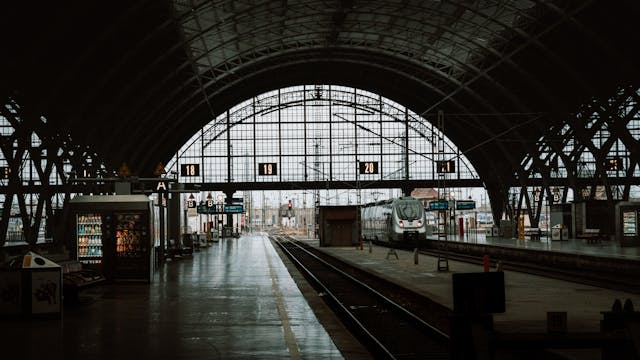
\includegraphics[width = 1\textwidth]{pics/image.jpeg}
    \caption{Cool train station}
    \label{fig: image1}
\end{figure*}

\begin{figure*}[htbp]
    \centering
    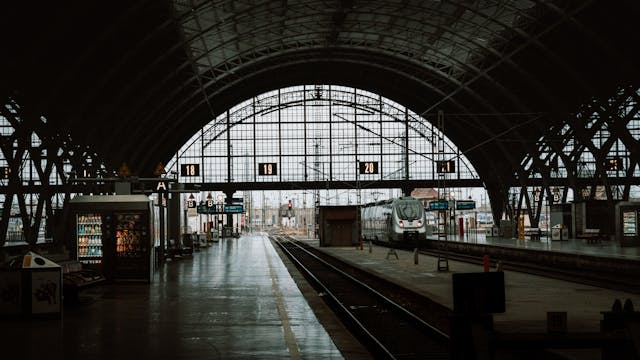
\includegraphics[width = 1\textwidth]{pics/image.jpeg}
    \caption{This cool train station stands as a metaphor for life itself, everyone's waiting, no one knows when their train will arrive, and someone's always holding the wrong ticket. Yet, we all stand here pretending everything's fine, sipping overpriced coffee with quiet determination}
    \label{fig: image2}
\end{figure*}

\begin{figure*}[htbp]
    \centering
    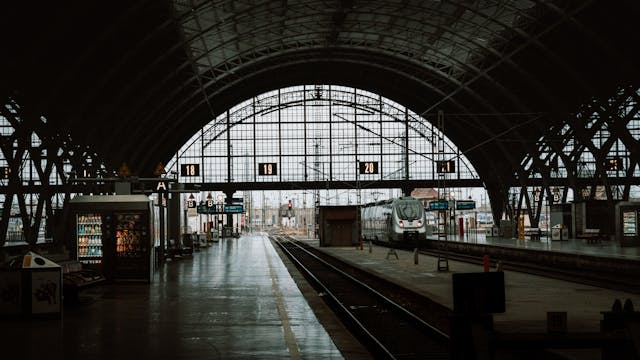
\includegraphics[width = 1\textwidth]{pics/image.jpeg}
    \caption{Cool train station}
    \label{fig: image2}
\end{figure*}

Content Text Content Text Content Text Content Text Content Text Content Text Content Text Content Text Content Text Content Text Content Text Content Text Content Text.

\begin{figure*}[htbp]
    \centering
    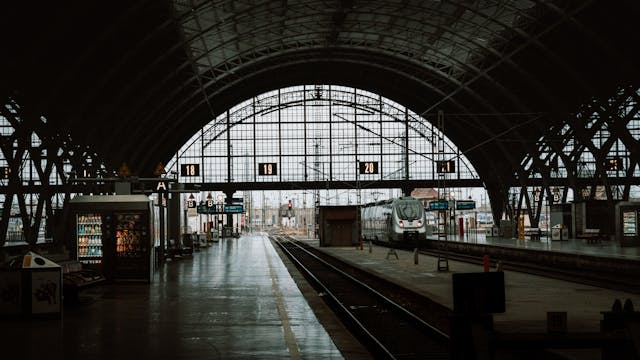
\includegraphics[width = 0.5\textwidth]{pics/image.jpeg}
    \caption{Cool train station}
    \label{fig: image}
\end{figure*}

\end{Chapter}
% 章節二 Chapter 2
\begin{Chapter}

\chapter{Title Example 2}

\section{Section Header Level 1}

Content Text Content Text Content Text Content Text Content Text Content Text Content \cite{knuth:1984} Text Content Text Content Text Content Text Content Text Content Text Content Text \cite{latex2e}, Content Text Content Text Content Text Content Text Content Text Content Text Content Text Content Text Content Text Content Text Content Text Content Text Content Text.

\begin{table*}[htbp]
    \centering
    \caption{Another table caption} \label{tab: complexity}
    \makebox[\linewidth][c]{
    \renewcommand\arraystretch{1.2}{
        \begin{tabular}{| l | c  c  c  c |}
        \hline
        Protocol & $P$ & $CS_1$ & $CS_2$ & $RG$ \\
        \hline
        MSSMul & $O(1)$, $O(1)$, N/A & $O(n-t)$, $O(n)$, $O(1)$ & $O(n-t)$, $O(n)$, N/A & $O(1)$, $O(n)$, $O(n)$ \\
        SC & $O(1)$, $O(1)$, N/A & $O(n-t)$, $O(n)$, $O(1)$ & $O(n-t)$, $O(n)$, N/A & $O(1)$, $O(n)$, $O(n)$ \\
        \hline 
        \end {tabular}
    }}
\end {table*}

\section{Section Header Level 1}

Content Text Content Text Content Text Content Text Content Text Content Text Content Text Content Text Content Text Content Text Content Text Content Text Content Text.

\begin{figure*}[htbp]
    \centering
    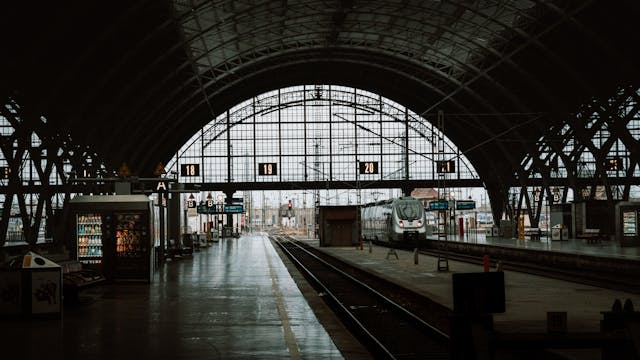
\includegraphics[width = 0.5\textwidth]{pics/image.jpeg}
    \caption{Cool train station}
    \label{fig: image}
\end{figure*}

\begin{figure}[ht]
    \centering
    \begin{minipage}{\linewidth}
        \centering
        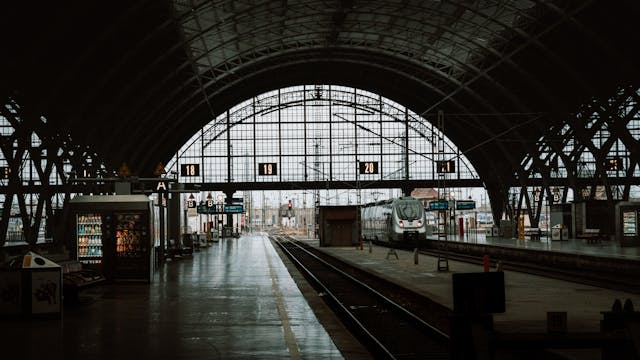
\includegraphics[width=\linewidth]{pics/image.jpeg}
        \vspace{0.5ex}
        \small (a)
    \end{minipage}
    \vspace{0.5em}
    
    \begin{minipage}{\linewidth}
        \centering
        \includegraphics[width=\linewidth]{pics/train-station2.jpeg}
        \vspace{0.5ex}
        \small (b)
    \end{minipage}
    \caption{Illustration of the train stations: (a) and (b) (Continued in Figure~\ref{fig2-cont})}
    \label{fig2}
\end{figure}

\begin{figure}[ht]
    \centering
    \begin{minipage}{\linewidth}
        \centering
        \includegraphics[width=\linewidth]{pics/train-station3.jpg}
        \vspace{0.5ex}
        \small (c)
    \end{minipage}
    \vspace{0.5em}
    
    \begin{minipage}{\linewidth}
        \centering
        \includegraphics[width=\linewidth]{pics/train-station4.jpg}
        \vspace{0.5ex}
        \small (d)
    \end{minipage}
    \caption{Illustration of the train stations: (c) and (d)}
    \label{fig2-cont}
\end{figure}

You may also, somehow, need to put a very looong table into your work, like "this one" \ref{sec.longtable}, which is fine, and I understand. Here's how you could put it like the table \ref{sec.longtable}

\begin{longtable}{|p{0.3\textwidth}|p{0.25\textwidth}|p{0.35\textwidth}|}
\caption{A very loooong table} \label{sec.longtable}\\
\hline
\textbf{Category}& \textbf{ID}& \multicolumn{1}{|c|}{\textbf{Comment}} \\
\hline
\endfirsthead

\hline
\multicolumn{3}{|c|}{Continuation of Table \ref{sec.longtable}}\\
\hline
\textbf{Category}& \textbf{ID}& \multicolumn{1}{|c|}{\textbf{Comment}} \\
\hline
\endhead

\hline
\endfoot

\hline
\multicolumn{3}{|c|}{End of Table \ref{sec.longtable}}\\\hline
\endlastfoot

\textbf{1\_Foo}& \textbf{Bar}& 0\_Foo \\
&&1\_Bar\\
&&2\_Foo\\
&&3\_Bar\\
&&4\_Foo\\
&&5\_Bar\\
&&6\_Foo\\
&&7\_Bar\\
&&8\_Foo\\
&&9\_Bar\\
&&10\_Foo\\
&&11\_Bar\\
\hline
\textbf{2\_Foo}& \textbf{Bar}&12\_Foo\\
&&13\_Bar\\
&&14\_Foo\\
&&15\_Bar\\
&&16\_Foo\\
&&17\_Bar\\
&&18\_Foo\\
&&19\_Bar\\
&&20\_Foo\\
&&21\_Bar\\
&&22\_Foo\\
&&23\_Bar\\
&&24\_Foo\\
&&25\_Bar\\
&&26\_Foo\\
&&27\_Bar\\
&&28\_Foo\\
&&29\_Bar\\
&&30\_Foo\\
&&31\_Bar\\
&&32\_Foo\\
&&33\_Bar\\
&&34\_Foo\\
&&35\_Bar\\
&&36\_Foo\\
&&37\_Bar\\
&&38\_Foo\\
&&39\_Bar\\
&&40\_Foo\\
&&41\_Bar\\
&&42\_Foo\\
&&43\_Bar\\
&&44\_Foo\\
&&45\_Bar\\
&&46\_Foo\\
&&47\_Bar\\
&&48\_Foo\\
\hline
\textbf{3\_Foo}&\textbf{Bar}&49\_Bar\\
&&50\_Foo\\
&&51\_Bar\\
&&52\_Foo\\
&&53\_Bar\\
&&54\_Foo\\
&&55\_Bar\\
&&56\_Foo\\
&&57\_Bar\\
&&58\_Foo\\
&&59\_Bar\\
\hline
\end{longtable}

\end{Chapter}
% 新增你自己的章節... Add chapters here

% 參考文獻,請在段落上隨意註解,你同時需要 reference.bib
\addcontentsline{toc}{chapter}{參考文獻}
\renewcommand{\bibname}{參考文獻}
\printbibliography


\end{document}
